\section{Technical Approaches}
The RoboNotts team has successfully competed in other competitions, most recently winning the METRICS HEART-MET Physically Assistive Robot Challenge~\cite{ref_url1} hosted at the IEEE International Conference for Robotics and Automation (ICRA) 2023 in London. The team received special recognition for their performance in human-robot interaction.

\subsection{Hardware Architecture}

\begin{wrapfigure}{r}{0.20\textwidth}
\centering
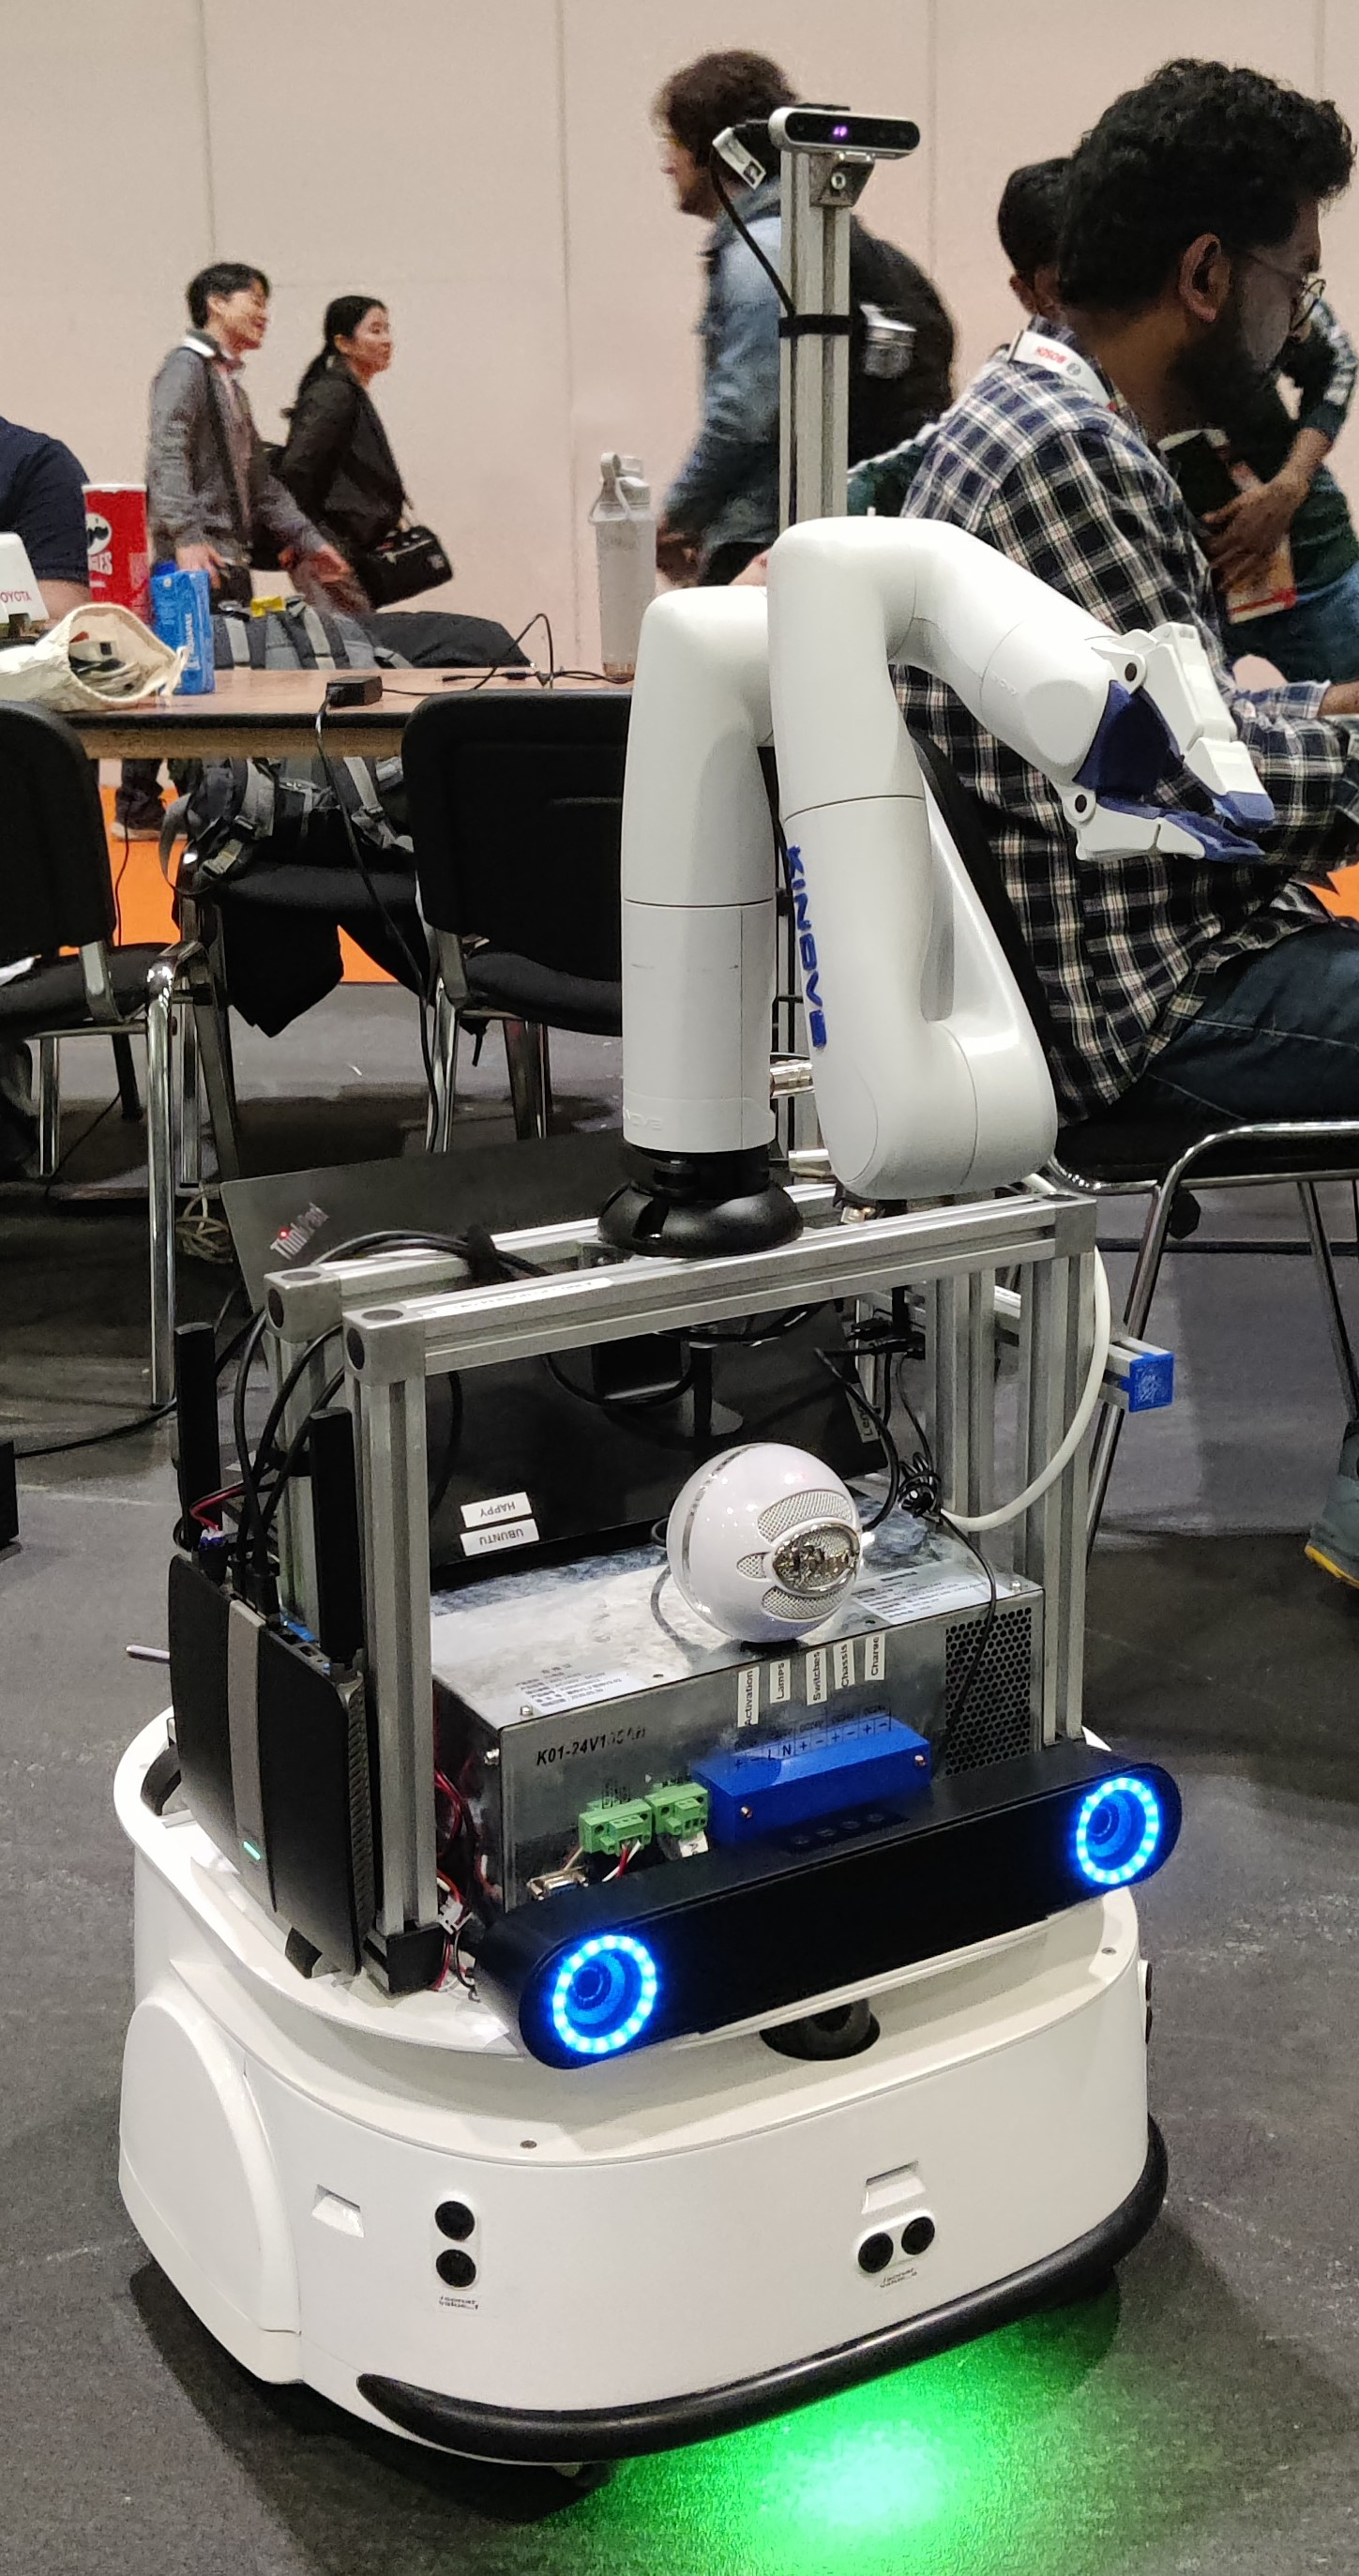
\includegraphics[scale=0.04]{HAPPY}
\caption{HAPPY at ICRA 2023.} \label{fig.1}
\end{wrapfigure}
The RoboNotts Team uses a custom-built adaptable platform, known as HAPPY. The HAPPY platform consists of a large base with a differential drive, Lidar, and other sensors useful in navigation. This base was originally part of a AMY-M2-W1 disinfection robot developed by AMY Robotics~\cite{ref_url2}. The team has built HAPPY up from this base, along with the necessary hardware required for benchmarks.

The team intends to continue building upon HAPPY, developing a flexible platform for investigating novel solutions. Currently, the team is working on developing a casing to improve the appearance of HAPPY.

\subsubsection{Actuators}

HAPPY has three main actuators, Two motors on the base that provide differential drive, and a Kinova Gen3 Lite robotic arm for manipulating objects.

\subsubsection{Sensors}

HAPPY is equipped with two Intel Realsense RGB-D cameras for image recognition and depth perception, a forward facing LiDaR, a pressure activated bump sensor that covers both the front and rear of the robot, two Infrared Drop Sensors, and 6 sonar sensors.

\subsection{Software Architecture}

HAPPY's software stack is built upon the Robotics Operating System (ROS). The RoboNotts team has successfully deployed a mix of existing and custom-developed ROS packages for benchmarks in the past.

These packages performed essential tasks, including object perception, navigation, speech recognition, and object manipulation. This year the team will be reworking a lot of the previous code to move to ROS2, as well as increasing HAPPY's capabilities by moving work from solved problems to unsolved problems. All the modules and more in-depth description of these can be found in the team's repositories~\cite{ref_git}. All of RoboNotts' development is free and open-source.

\subsubsection{Low-Level Software}

The robotic base from AMY Robotics originally came pre-installed with ROS Indigo. The proprietary and outdated code for the base, and it's odd implementation has severely limited the team in the past. In order to rectify this, the team has rewritten the entire code for the base from scratch for ROS2 Iron. This a massive technical feat, and will give more flexibility in building out the team's work.

\subsubsection{Computer Vision}

We have two main computer vision models that we use in rotation, an off the shelf YOLO~\cite{yolo} model and a custom FCOS~\cite{fcos} model implementation. Either can be used for computer vision with each offering strengths and are then trained on custom built datasets fit for each competition. Should further segmentation be needed, e.g. for manipulation tasks, we can then pass the bounding boxes as prompts for a pre-trained Segment Anything Model~\cite{sam}.

For tasks that require person detection, pose estimation, activity detection, etc. we use MediaPipe~\cite{mp}, as well as custom AI models using TensorFlow~\cite{tf}.

\subsubsection{Navigation}

To achieve effective navigation, RoboNotts uses the Slam Toolbox~\cite{slamtb} and Nav2 ROS package~\cite{nav2}. HAPPY's LiDAR and range sensors are used to create a base map of an area, to which important details are added; way-points (areas often traversed) for navigation, locations of interest (such as the position of doors, or where sitting areas are), and start/end positions for benchmarks. Once this refined map is built, the Nav2 navigation stack is used to traverse between these points, effectively building a graph-based map of an area.
Object avoidance is performed proactively by the Nav2 stack, but the team also produced ROS nodes which are tasked with reactive object avoidance in the case of unexpected obstacles. These nodes work by detecting objects not only with the range-finders, but also with the depth cameras, assuring that the robot never collides with any objects. 

\subsubsection{Human-Robot Interaction} 

The team's approach to Human-Robot Interaction involves the use of multiple steps.

\begin{figure}
    \centering
    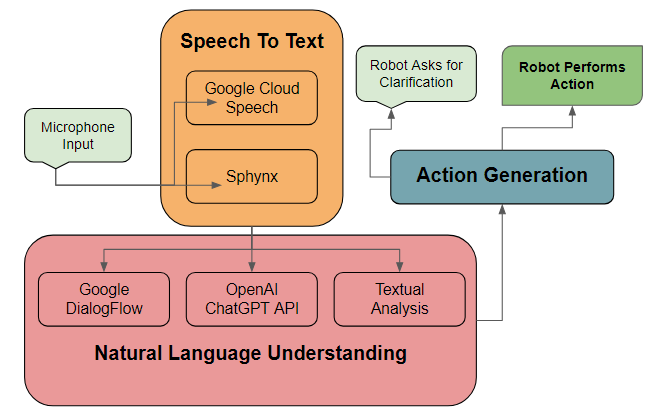
\includegraphics[scale=0.40]{HRI.png}
    \caption{RoboNotts HRI Pipeline} \label{fig.1}
\end{figure}

\begin{enumerate}
    \item Utilisation of Google Cloud Speech and Sphinx Speech facilitates the extraction speech from microphone input, transcribing it into text.
    \item Semantic information is then extracted from the generated text through the following steps:
    \begin{enumerate}
        \item The text undergoes analysis using a Google DialogFlow pipeline explicitly crafted for the detection and extraction of actions. This pipeline is adept at accommodating synonymous expressions. Instances of common actions, such as "Fetch me the bottle," are processed into a structured command format, for instance: "FETCH \{item=bottle\}".
        \item Textual content that cannot be comprehended by DialogFlow is routed through a finely-tuned iteration of OpenAI's ChatGPT. This language model is entrusted with extracting meanings and, if applicable, generating a contextually appropriate response in the event that the understood text is neither a command nor an anticipated statement (e.g., "What is your favourite item?").
        \item In instances where the aforementioned methods prove ineffective, we query a large library of words associated with actions, attempting to infer the intended action. While this is inefficient and prone to failure, this approach may avoid needing to repeat questions. 
    \end{enumerate}
    If a discernible action is successfully derived, it is subsequently directed to a designated node responsible for executing the associated actions. In cases where neither an actionable command nor an apt response can be ascertained, the robot asks the user to clarify their command. To enhance the likeability of the robot, the team leverages ChatGPT to generate diverse and unique responses, thereby mitigating the recurrence of identical sentences.
\end{enumerate}
